\documentclass[11pt]{article}
%Gummi|065|=)

%%%%%%%%%%%%%%%%%%%%%%%%%%%%%%%%%%%%%%%%%%%%%%%%%%%%%%%%%%%%%%%%%%%%%%%%%%%%%
\usepackage[utf8]{inputenc}
\usepackage[english]{babel}

%%%%%%%%%%%%%%%%%%%%%%%%%%%%%%%%%%%%%%%%%%%%%%%%%%%%%%%%%%%%%%%%%%%%%%%%%%%%%
\usepackage{amsmath}
\usepackage{amsfonts}
\usepackage{amssymb}
\usepackage{graphicx}
\usepackage{mathtools}

%%%%%%%%%%%%%%%%%%%%%%%%%%%%%%%%%%%%%%%%%%%%%%%%%%%%%%%%%%%%%%%%%%%%%%%%%%%%%
\usepackage{verbatim} % para \begin{comment}

%%%%%%%%%%%%%%%%%%%%%%%%%%%%%%%%%%%%%%%%%%%%%%%%%%%%%%%%%%%%%%%%%%%%%%%%%%%%%
\newcommand{\transpose}{\mathrm{T}}

%%% \newcommand{COMANDO}[ARGUMENTOS]{DEFINICIÓN}
%\newcommand{\TRIX}[1]{\mathbf{\overline{\overline{\overline{\lowercase{#1}}}}}}
%\newcommand{\MATRIX}[1]{\mathbf{\overline{\overline{\lowercase{#1}}}}}
%\newcommand{\VECTOR}[1]{\mathbf{\overline{\lowercase{#1}}}}
\newcommand{\TRIX}[1]{\mathbf{\overline{\uppercase{#1}}}}
\newcommand{\MATRIX}[1]{\mathbf{\uppercase{#1}}}
\newcommand{\VECTOR}[1]{\mathbf{\lowercase{#1}}}


\newcommand{\mulebe}{\circledast}
\newcommand{\mulinner}{\odot}
\newcommand{\mulcross}{\otimes}
\newcommand{\dimsep}{,}

\newcommand{\mulcrossxy}{\mulcross_{e_1}^{e_2}}
\newcommand{\mulcrossyz}{\mulcross_{e_2}^{e_3}}
\newcommand{\mulcrossxz}{\mulcross_{e_1}^{e_3}}

\newcommand{\mulcrossyx}{\mulcross_{e_2}^{e_1}}
\newcommand{\mulcrosszy}{\mulcross_{e_3}^{e_2}}
\newcommand{\mulcrosszx}{\mulcross_{e_3}^{e_1}}


\newcommand{\funcmuliiinner}{inner_3 }
\newcommand{\funcmulcccross}{cross_3 }


%%%%%%%%%%%%%%%%%%%%%%%%%%%%%%%%%%%%%%%%%%%%%%%%%%%%%%%%%%%%%%%%%%%%%%%%%%%%%
\newtheorem{theorem}{Theorem}
\newtheorem{definition}{Definition}

%%%%%%%%%%%%%%%%%%%%%%%%%%%%%%%%%%%%%%%%%%%%%%%%%%%%%%%%%%%%%%%%%%%%%%%%%%%%%
\title{\textbf{Trix: Arrays in 3D}}
\author{Fernando Pujaico Rivera}
\date{}
\begin{document}

\maketitle

%%%%%%%%%%%%%%%%%%%%%%%%%%%%%%%%%%%%%%%%%%%%%%%%%%%%%%%%%%%%%%%%%%%%%%%%%%%%%%%%%%%%%%%%%%%%%%%%%
%%%%%%%%%%%%%%%%%%%%%%%%%%%%%%%%%%%%%%%%%%%%%%%%%%%%%%%%%%%%%%%%%%%%%%%%%%%%%%%%%%%%%%%%%%%%%%%%%
\section{Definitions}
\begin{definition}\label{def:vector}
A vector $\VECTOR{a}\in \mathbb{R}^{M}$ is an array in $1D$, with elements $a_{m}$, 
$\{m\}\in \mathbb{N}$, $1 \leq m \leq M$.Example:
\begin{equation}
 a_{:}\equiv \VECTOR{a}=\{a_1~\hdots~a_m~\hdots~a_{M} \}
\end{equation}
Where $\{~\}$ indicates a grouping in one dimension. 
\end{definition}

\begin{definition}\label{def:matrix}
A matrix $\MATRIX{B}\in \mathbb{R}^{M\dimsep N }$ is an array in $2D$, with elements $b_{mn}$, 
$\{m,n\}\in\mathbb{N}$, $1 \leq m \leq M$, $1 \leq n \leq N$.Example:
\begin{equation}
 b_{::}\equiv \MATRIX{B}=\left[
 \begin{matrix}
 b_{11} &\hdots &b_{1m} &\hdots &b_{1N}\\ 
 b_{21} &\hdots &b_{2m} &\hdots &b_{2N}\\
 \vdots &\vdots &\vdots &\vdots &\vdots\\ 
 b_{M1} &\hdots &b_{Mm} &\hdots &b_{MN}\\ 
 \end{matrix}
 \right]
\end{equation}
Where $[~]$ indicates a grouping in two dimensions. 
\end{definition}

\begin{definition}\label{def:trix}
A trix $\TRIX{C}\in \mathbb{R}^{M\dimsep N\dimsep L}$ is an array in $3D$, with elements $c_{mnl}$, 
$\{m,n,l\}\in\mathbb{N}$, $1 \leq m \leq M$, $1 \leq n \leq N$, $1 \leq l \leq L$.Example:
\begin{equation}
 c_{::l}=\left[
 \begin{matrix}
 c_{11l} &\hdots &c_{1ml} &\hdots &c_{1Nl}\\ 
 c_{21l} &\hdots &c_{2ml} &\hdots &c_{2Nl}\\
 \vdots &\vdots &\vdots &\vdots &\vdots\\ 
 c_{M1l} &\hdots &c_{Mml} &\hdots &c_{MNl}\\ 
 \end{matrix}
 \right]
\end{equation}
\begin{equation}
c_{:::}\equiv \TRIX{C}=\left(
 \begin{matrix}
 c_{::1}&\hdots&c_{::l}&\hdots&c_{::L}\\
 \end{matrix}
 \right)
\end{equation}
Where $(~)$ indicates a grouping in the dimension of the variable, in this case $l$. 
By example, the Fig. \ref{fig:trixC} represents a trix $\TRIX{C}\in \mathbb{R}^{M\dimsep N\dimsep L}$.
Where $e_1$, $e_2$ and $e_3$ indicate the axes $1$, $2$ and $3$, respectively.
\begin{figure}[h]
  \centering
    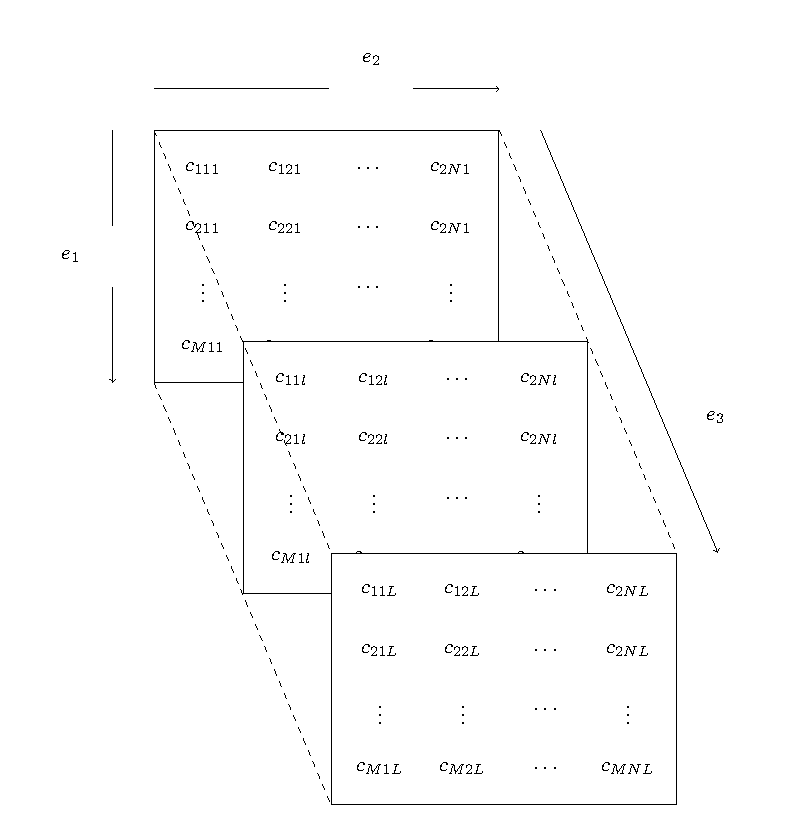
\includegraphics[width=0.8\textwidth]{trix-img}
    \caption{Trix C}
    \label{fig:trixC}
\end{figure}

\end{definition}

The Table \ref{tab:table1} show the notation of variable types used in this work,
following the Definitions \ref{def:vector}, \ref{def:matrix} and \ref{def:trix}.
\begin{table}[!ht]
  \centering
  \begin{tabular}{l|l|l}
  Notation     & Name   & Range \\ \hline
  $\alpha$, $\beta$, $\dots$      & Scalar & $\mathbb{R}$\\
  $\VECTOR{a}$, $\VECTOR{b}$, $\dots$ & Vector & $\mathbb{R}^{M}$\\
  $\MATRIX{A}$, $\MATRIX{B}$, $\dots$ & Matrix & $\mathbb{R}^{M \dimsep N}$\\
  $\TRIX{A}$, $\TRIX{B}$, $\dots$   & Trix   & $\mathbb{R}^{M \dimsep N \dimsep L}$\\
  \end{tabular}
  \caption{Notation of variable types used.}
  \label{tab:table1}
\end{table}

%%%%%%%%%%%%%%%%%%%%%%%%%%%%%%%%%%%%%%%%%%%%%%%%%%%%%%%%%%%%%%%%%%%%%%%%%%%%%%%%%%%%%%%%%%%%%%%%%
%%%%%%%%%%%%%%%%%%%%%%%%%%%%%%%%%%%%%%%%%%%%%%%%%%%%%%%%%%%%%%%%%%%%%%%%%%%%%%%%%%%%%%%%%%%%%%%%%
\newpage
\section{Operations until $\mathbb{R}$}

\subsection{Element by element operation : $\alpha\mulebe \beta \equiv \beta\mulebe \alpha$}
  $\mathbb{R}\mulebe \mathbb{R}$ $\rightarrow \mathbb{R}$.  Multiplication element by element
  in the case of real numbers $\alpha\mulebe \beta \equiv \alpha \beta$ given that exist only one element.  


%%%%%%%%%%%%%%%%%%%%%%%%%%%%%%%%%%%%%%%%%%%%%%%%%%%%%%%%%%%%%%%%%%%%%%%%%%%%%%%%%%%%%%%%%%%%%%%%%
%%%%%%%%%%%%%%%%%%%%%%%%%%%%%%%%%%%%%%%%%%%%%%%%%%%%%%%%%%%%%%%%%%%%%%%%%%%%%%%%%%%%%%%%%%%%%%%%%
\newpage\
\section{Operations until $\mathbb{R}^{M}$}

\subsection{Element by element operation : $\alpha\mulebe \VECTOR{a} \equiv \VECTOR{a} \mulebe \alpha$}
  $\mathbb{R}\mulebe \mathbb{R}^{M}$ $\rightarrow \mathbb{R}^{M}$.  Multiplication element by element 
  between two operators of different dimensions, the operator of less dimension is upgrade by 
  successive repetition. Result:
  $\{\alpha~\hdots~\alpha \}\mulebe \{a_1~\hdots~a_{M} \}\equiv \{\alpha a_1~\hdots~\alpha a_{M} \}$

\subsection{Element by element operation : $\VECTOR{a} \mulebe \VECTOR{b} \equiv \VECTOR{b} \mulebe \VECTOR{a}$}
  $\mathbb{R}^{M} \mulebe \mathbb{R}^{M}$ $\rightarrow \mathbb{R}^{M}$.  Multiplication element by element 
  between two operators. Result:
  $\{a_1~\hdots~a_{M} \}\mulebe \{b_1~\hdots~b_{M} \}\equiv \{a_1 b_1~\hdots~a_{M} b_{M} \}$
  
\subsection{Inner operation : $\VECTOR{a}\mulinner \VECTOR{b}\equiv \VECTOR{b}\mulinner \VECTOR{a}$}
 
  $\mathbb{R}^{M}\mulinner \mathbb{R}^{M}$ $\rightarrow \mathbb{R}$.  Dot product or multiplication element by element 
  between two operators and summation of all elements . 
  Result: 
  \begin{equation}
\sum \limits_{m=1}^{M} {a_m b_m}=sum\left( \VECTOR{a} \mulebe \VECTOR{b} \right)
  \end{equation}
  
\subsection{Inner operation : $\funcmuliiinner ( \VECTOR{a}, \VECTOR{b}, \VECTOR{c})$}
 
  $\funcmuliiinner( \mathbb{R}^{M}, \mathbb{R}^{M}, \mathbb{R}^{M})$ 
  $\rightarrow \mathbb{R}$.  Dot product or multiplication element by element 
  between three operators and summation of all elements . 
  Result: 
  \begin{equation}
\funcmuliiinner( \VECTOR{a}, \VECTOR{b}, \VECTOR{c})=
\sum \limits_{m=1}^{M} {a_m b_m c_m}=sum\left( \VECTOR{a} \mulebe \VECTOR{b}  \mulebe \VECTOR{c}\right)
  \end{equation}  

%%%%%%%%%%%%%%%%%%%%%%%%%%%%%%%%%%%%%%%%%%%%%%%%%%%%%%%%%%%%%%%%%%%%%%%%%%%%%%%%%%%%%%%%%%%%%%%%%
%%%%%%%%%%%%%%%%%%%%%%%%%%%%%%%%%%%%%%%%%%%%%%%%%%%%%%%%%%%%%%%%%%%%%%%%%%%%%%%%%%%%%%%%%%%%%%%%%
\newpage\
\section{Operations until $\mathbb{R}^{M \dimsep N}$}

\subsection{Element by element operation : $\alpha\mulebe  \MATRIX{B}\equiv \MATRIX{B}\mulebe \alpha$}

 $\mathbb{R}\mulebe \mathbb{R}^{M\dimsep N}$ $\rightarrow \mathbb{R}^{M\dimsep N}$.Multiplication element by element 
  between two operators of different dimensions, the operator of less dimension is upgrade by 
  successive repetition. Result: 
\begin{equation}
  \left[
 \begin{matrix}
 \alpha &\hdots &\alpha\\ 
 \alpha &\hdots &\alpha\\
 \vdots &\vdots &\vdots\\ 
 \alpha &\hdots &\alpha\\ 
 \end{matrix}
 \right]\mulebe 
   \left[
 \begin{matrix}
 b_{11} &\hdots &b_{1N}\\ 
 b_{21} &\hdots &b_{2N}\\
 \vdots &\vdots &\vdots\\ 
 b_{M1} &\hdots &b_{MN}\\ 
 \end{matrix}
 \right]
 \equiv \left[
 \begin{matrix}
 \alpha b_{11} &\hdots &\alpha b_{1N}\\ 
 \alpha b_{21} &\hdots &\alpha b_{2N}\\
 \vdots &\vdots &\vdots\\ 
 \alpha b_{M1} &\hdots &\alpha b_{MN}\\ 
 \end{matrix}
 \right]
 \end{equation}

\begin{comment}
\subsection{Element by element operation : $\VECTOR{a}^{e_1}\mulebe  \MATRIX{B}\equiv \MATRIX{B}\mulebe \VECTOR{a}^{e_1} $}
$\mathbb{R}^M\mulebe \mathbb{R}^{M\dimsep N}$ $\rightarrow \mathbb{R}^{M\dimsep N}$. 
Multiplication element by element 
  between two operators of different dimensions, 
  the operator of less dimension is upgrade by successive repetition of $\VECTOR{a}$ as $e_1$ (column matrix) in $e_2$ (second axes). Result: 
\begin{equation}
  \left[
 \begin{matrix}
 a_{1} &\hdots &a_{1}\\ 
 a_{2} &\hdots &a_{2}\\
 \vdots &\vdots &\vdots\\ 
 a_{M} &\hdots &a_{M}\\ 
 \end{matrix}
 \right]\mulebe 
   \left[
 \begin{matrix}
 b_{11} &\hdots &b_{1N}\\ 
 b_{21} &\hdots &b_{2N}\\
 \vdots &\vdots &\vdots\\ 
 b_{M1} &\hdots &b_{MN}\\ 
 \end{matrix}
 \right]
 \equiv \left[
 \begin{matrix}
 a_{1} b_{11} &\hdots &a_{1} b_{1N}\\ 
 a_{2} b_{21} &\hdots &a_{2} b_{2N}\\
 \vdots &\vdots &\vdots\\ 
 a_{M} b_{M1} &\hdots &a_{M} b_{MN}\\ 
 \end{matrix}
 \right]
 \end{equation}

\subsection{Element by element operation : $\VECTOR{a}^{e_2}\mulebe  \MATRIX{B}\equiv \MATRIX{B}\mulebe \VECTOR{a}^{e_2} $}
$\mathbb{R}^N\mulebe \mathbb{R}^{M\dimsep N}$ $\rightarrow \mathbb{R}^{M\dimsep N}$.
Multiplication element by element 
  between two operators of different dimensions, 
  the operator of less dimension is upgrade by successive repetition of $\VECTOR{a}$ as $e_2$ (row matrix) in $e_1$ (first axes). Result: 
\begin{equation}
  \left[
 \begin{matrix}
 a_{1} &\hdots &a_{N}\\ 
 a_{1} &\hdots &a_{N}\\
 \vdots &\vdots &\vdots\\ 
 a_{1} &\hdots &a_{N}\\ 
 \end{matrix}
 \right]\mulebe 
   \left[
 \begin{matrix}
 b_{11} &\hdots &b_{1N}\\ 
 b_{21} &\hdots &b_{2N}\\
 \vdots &\vdots &\vdots\\ 
 b_{M1} &\hdots &b_{MN}\\ 
 \end{matrix}
 \right]
 \equiv \left[
 \begin{matrix}
 a_{1} b_{11} &\hdots &a_{N} b_{1N}\\ 
 a_{1} b_{21} &\hdots &a_{N} b_{2N}\\
 \vdots &\vdots &\vdots\\ 
 a_{1} b_{M1} &\hdots &a_{N} b_{MN}\\ 
 \end{matrix}
 \right]
 \end{equation}
 
\end{comment}
 
\subsection{Element by element operation : $\MATRIX{A}\mulebe  \MATRIX{B}\equiv \MATRIX{B}\mulebe \MATRIX{A} $}
$\mathbb{R}^{M\dimsep N}\mulebe \mathbb{R}^{M\dimsep N}$ $\rightarrow \mathbb{R}^{M\dimsep N}$.
Multiplication element by element 
  between two operators.
Result: 
\begin{equation}
  \left[
 \begin{matrix}
 a_{11} &\hdots &a_{1N}\\ 
 a_{21} &\hdots &a_{2N}\\
 \vdots &\vdots &\vdots\\ 
 a_{M1} &\hdots &a_{MN}\\ 
 \end{matrix}
 \right]\mulebe 
   \left[
 \begin{matrix}
 b_{11} &\hdots &b_{1N}\\ 
 b_{21} &\hdots &b_{2N}\\
 \vdots &\vdots &\vdots\\ 
 b_{M1} &\hdots &b_{MN}\\ 
 \end{matrix}
 \right]
 \equiv \left[
 \begin{matrix}
 a_{11} b_{11} &\hdots &a_{1N} b_{1N}\\ 
 a_{21} b_{21} &\hdots &a_{2N} b_{2N}\\
 \vdots &\vdots &\vdots\\ 
 a_{M1} b_{M1} &\hdots &a_{MN} b_{MN}\\ 
 \end{matrix}
 \right]
 \end{equation}

\subsection{Inner operation : $\MATRIX{A}\mulinner \MATRIX{B}\equiv \MATRIX{B}\mulinner \MATRIX{A} $}
$\mathbb{R}^{M\dimsep N}. \mathbb{R}^{M\dimsep N}$ $\rightarrow \mathbb{R}$.
Result: 
  \begin{equation}
\MATRIX{A}\mulinner \MATRIX{B} = \sum \limits_{m=1}^{M}\sum \limits_{n=1}^{N} {a_{mn} b_{mn}} = sum\left(\MATRIX{A}\mulebe  \MATRIX{B}\right)
  \end{equation}
  

\subsection{Cross operation : $\MATRIX{A}\mulcross \MATRIX{B}\equiv \MATRIX{A}\mulcrossyx \MATRIX{B}$}
$\mathbb{R}^{M\dimsep P}\mulcross \mathbb{R}^{P\dimsep N}$ $\rightarrow \mathbb{R}^{M\dimsep N}$
that is equivalent to
$\mathbb{R}^{M\dimsep P}\mulcrossyx \mathbb{R}^{P\dimsep N}$ $\rightarrow \mathbb{R}^{M\dimsep N}$.
Result: 
  \begin{equation}
\MATRIX{A}\mulcross \MATRIX{B}
 \equiv \left[
 \begin{matrix}
 a_{1:}\mulinner b_{:1} &\hdots &a_{1:}\mulinner b_{:N}\\ 
 a_{2:}\mulinner b_{:1} &\hdots &a_{2:}\mulinner b_{:N}\\
 \vdots &\vdots &\vdots\\ 
 a_{M:}\mulinner b_{:1} &\hdots &a_{M:}\mulinner b_{:N}\\ 
 \end{matrix}
 \right]
  \end{equation}

\subsection{Cross operation : $\MATRIX{A}\mulcrossxy \MATRIX{B}$}
$\mathbb{R}^{P\dimsep M}\mulcross \mathbb{R}^{N\dimsep P}$ $\rightarrow \mathbb{R}^{M\dimsep N}$
  \begin{equation}
\MATRIX{A}\mulcrossxy \MATRIX{B}
 \equiv \left[
 \begin{matrix}
 a_{:1}\mulinner b_{1:} &\hdots &a_{:1}\mulinner b_{N:}\\ 
 a_{:2}\mulinner b_{1:} &\hdots &a_{:2}\mulinner b_{N:}\\
 \vdots &\vdots &\vdots\\ 
 a_{:M}\mulinner b_{1:} &\hdots &a_{:M}\mulinner b_{N:}\\ 
 \end{matrix}
 \right] \equiv \left \{\MATRIX{B}\mulcross \MATRIX{A} \right \}^{\transpose}
\equiv \MATRIX{A}^{\transpose}\mulcross \MATRIX{B}^{\transpose}
 \end{equation}
  
%%%%%%%%%%%%%%%%%%%%%%%%%%%%%%%%%%%%%%%%%%%%%%%%%%%%%%%%%%%%%%%%%%%%%%%%%%%%%%%%%%%%%%%%%%%%%%%%%
%%%%%%%%%%%%%%%%%%%%%%%%%%%%%%%%%%%%%%%%%%%%%%%%%%%%%%%%%%%%%%%%%%%%%%%%%%%%%%%%%%%%%%%%%%%%%%%%%
\newpage\
\section{Operations until $\mathbb{R}^{M \dimsep N \dimsep L}$}


\subsection{Element by element operation : $\alpha \mulebe  \TRIX{B}\equiv \TRIX{B}\mulebe \alpha$}

 $\mathbb{R}\mulebe \mathbb{R}^{M\dimsep N \dimsep L}$ $\rightarrow \mathbb{R}^{M\dimsep N \dimsep L}$.
 Multiplication element by element 
  between two operators of different dimensions, the operator of less dimension is upgrade by 
  successive repetition. Result: 
\begin{equation}
  \left[
 \begin{matrix}
 \alpha &\hdots &\alpha\\ 
 \alpha &\hdots &\alpha\\
 \vdots &\vdots &\vdots\\ 
 \alpha &\hdots &\alpha\\ 
 \end{matrix}
 \right]\mulebe 
   \left[
 \begin{matrix}
 b_{11l} &\hdots &b_{1Nl}\\ 
 b_{21l} &\hdots &b_{2Nl}\\
 \vdots &\vdots &\vdots\\ 
 b_{M1l} &\hdots &b_{MNl}\\ 
 \end{matrix}
 \right]
 \equiv \left[
 \begin{matrix}
 \alpha b_{11l} &\hdots &\alpha b_{1Nl}\\ 
 \alpha b_{21l} &\hdots &\alpha b_{2Nl}\\
 \vdots &\vdots &\vdots\\ 
 \alpha b_{M1l} &\hdots &\alpha b_{MNl}\\ 
 \end{matrix}
 \right]=c_{::l}
 \end{equation}

 \begin{equation}
\TRIX{C}=\left(
 \begin{matrix}
 c_{::1}&\hdots&c_{::l}&\hdots&c_{::L}\\
 \end{matrix}
 \right)
\end{equation}


\subsection{Element by element operation : $\TRIX{A} \mulebe  \TRIX{B}\equiv \TRIX{B}\mulebe \TRIX{A}$}

 $\mathbb{R}^{M\dimsep N \dimsep L} \mulebe \mathbb{R}^{M\dimsep N \dimsep L}$ 
 $\rightarrow \mathbb{R}^{M\dimsep N \dimsep L}$.
 Multiplication element by element between two operators. Result: 
\begin{equation}
  \left[
 \begin{matrix}
 a_{11l} &\hdots &a_{1Nl}\\ 
 a_{21l} &\hdots &a_{2Nl}\\
 \vdots &\vdots &\vdots\\ 
 a_{M1l} &\hdots &a_{MNl}\\ 
 \end{matrix}
 \right]\mulebe 
   \left[
 \begin{matrix}
 b_{11l} &\hdots &b_{1Nl}\\ 
 b_{21l} &\hdots &b_{2Nl}\\
 \vdots &\vdots &\vdots\\ 
 b_{M1l} &\hdots &b_{MNl}\\ 
 \end{matrix}
 \right]
 \equiv \left[
 \begin{matrix}
 a_{11l} b_{11l} &\hdots &a_{1Nl} b_{1Nl}\\ 
 a_{21l} b_{21l} &\hdots &a_{2Nl} b_{2Nl}\\
 \vdots &\vdots &\vdots\\ 
 a_{M1l} b_{M1l} &\hdots &a_{MNl} b_{MNl}\\ 
 \end{matrix}
 \right]=c_{::l}
 \end{equation}

 \begin{equation}
\TRIX{C}=\left(
 \begin{matrix}
 c_{::1}&\hdots&c_{::l}&\hdots&c_{::L}\\
 \end{matrix}
 \right)
\end{equation}



\subsection{Inner operation : $\TRIX{A} \mulinner \TRIX{B}\equiv \TRIX{B} \mulinner \TRIX{A}$}

 $\mathbb{R}^{M\dimsep N \dimsep L} \mulinner \mathbb{R}^{M\dimsep N \dimsep L}$ 
 $\rightarrow \mathbb{R}$.
 Inner product between two operators. Result: 
  \begin{equation}
\TRIX{A}\mulinner \TRIX{B} = \sum \limits_{m=1}^{M}\sum \limits_{n=1}^{N}\sum \limits_{l=1}^{L} {a_{mnl} b_{mnl}} = sum\left(\TRIX{A}\mulebe  \TRIX{B}\right)
  \end{equation}

 \subsection{Inner operation : $\funcmuliiinner( \TRIX{A},\TRIX{B}, \TRIX{C})$}

 $\funcmuliiinner(\mathbb{R}^{M\dimsep N \dimsep L}, \mathbb{R}^{M\dimsep N \dimsep L}, \mathbb{R}^{M\dimsep N \dimsep L})$ 
 $\rightarrow \mathbb{R}$.
 Inner product between 3 operators. Result: 
  \begin{equation}
\funcmuliiinner( \TRIX{A},\TRIX{B}, \TRIX{C}) = 
\sum \limits_{m=1}^{M}\sum \limits_{n=1}^{N}\sum \limits_{l=1}^{L} {a_{mnl} b_{mnl} c_{mnl}} = 
sum\left(\TRIX{A}\mulebe  \TRIX{B}\mulebe  \TRIX{C}\right)
  \end{equation}
  
\subsection{Cross operation : $\TRIX{A} \mulcrossyx \TRIX{B}$}
$\mathbb{R}^{M\dimsep P\dimsep L}\mulcrossyx \mathbb{R}^{P\dimsep N\dimsep L}$ $\rightarrow \mathbb{R}^{M\dimsep N\dimsep L}$.
Result: 
  \begin{equation}
  a_{::l}\mulcross b_{::l} \equiv c_{::l}
  \end{equation}
 \begin{equation}
\TRIX{C}=\TRIX{A} \mulcrossyx \TRIX{B} \equiv \left(
 \begin{matrix}
 c_{::1}&\hdots&c_{::l}&\hdots&c_{::L}\\
 \end{matrix}
 \right)
\end{equation}

\subsection{Cross operation : $\TRIX{A} \mulcrosszy \TRIX{B}$}
$\mathbb{R}^{M\dimsep N\dimsep P}\mulcrosszy \mathbb{R}^{M \dimsep P\dimsep L}$ $\rightarrow \mathbb{R}^{M\dimsep N\dimsep L}$.
Result: 
  \begin{equation}
  a_{m::}\mulcross b_{m::} \equiv c_{m::}
  \end{equation}
 \begin{equation}
\TRIX{C}=\TRIX{A} \mulcrosszy \TRIX{B} \equiv \left(
 \begin{matrix}
 c_{1::}&\hdots&c_{m::}&\hdots&c_{M::}\\
 \end{matrix}
 \right)
\end{equation}

\subsection{Cross operation : $\TRIX{A} \mulcrosszx \TRIX{B}$}
$\mathbb{R}^{M\dimsep N\dimsep P}\mulcrosszy \mathbb{R}^{P \dimsep N\dimsep L}$ $\rightarrow \mathbb{R}^{M\dimsep N\dimsep L}$.
Result: 
  \begin{equation}
  a_{:n:}\mulcross b_{:n:} \equiv c_{:n:}
  \end{equation}
 \begin{equation}
\TRIX{C}=\TRIX{A} \mulcrosszx \TRIX{B} \equiv \left(
 \begin{matrix}
 c_{:1:}&\hdots&c_{:n:}&\hdots&c_{:N:}\\
 \end{matrix}
 \right)
\end{equation}
  
  
\subsection{Cross operation : $\funcmulcccross(\MATRIX{A},\MATRIX{B},\MATRIX{C})$}
$\funcmulcccross(\mathbb{R}^{M \dimsep P \dimsep L}, \mathbb{R}^{P \dimsep N \dimsep L}, \mathbb{R}^{M \dimsep N \dimsep P})$ 
$\rightarrow \mathbb{R}^{M\dimsep N\dimsep L}$
  \begin{equation}
\TRIX{D} = \funcmulcccross(\TRIX{A},\TRIX{B},\TRIX{C})
 \end{equation}
  
  \begin{equation}
d_{mnl} = \funcmuliiinner( a_{m:l},b_{:nl}, c_{mn:})
 \end{equation}
  
This operation can be seen in the Fig. \ref{fig:trixcross3C}.
  \begin{figure}[h]
  \centering
    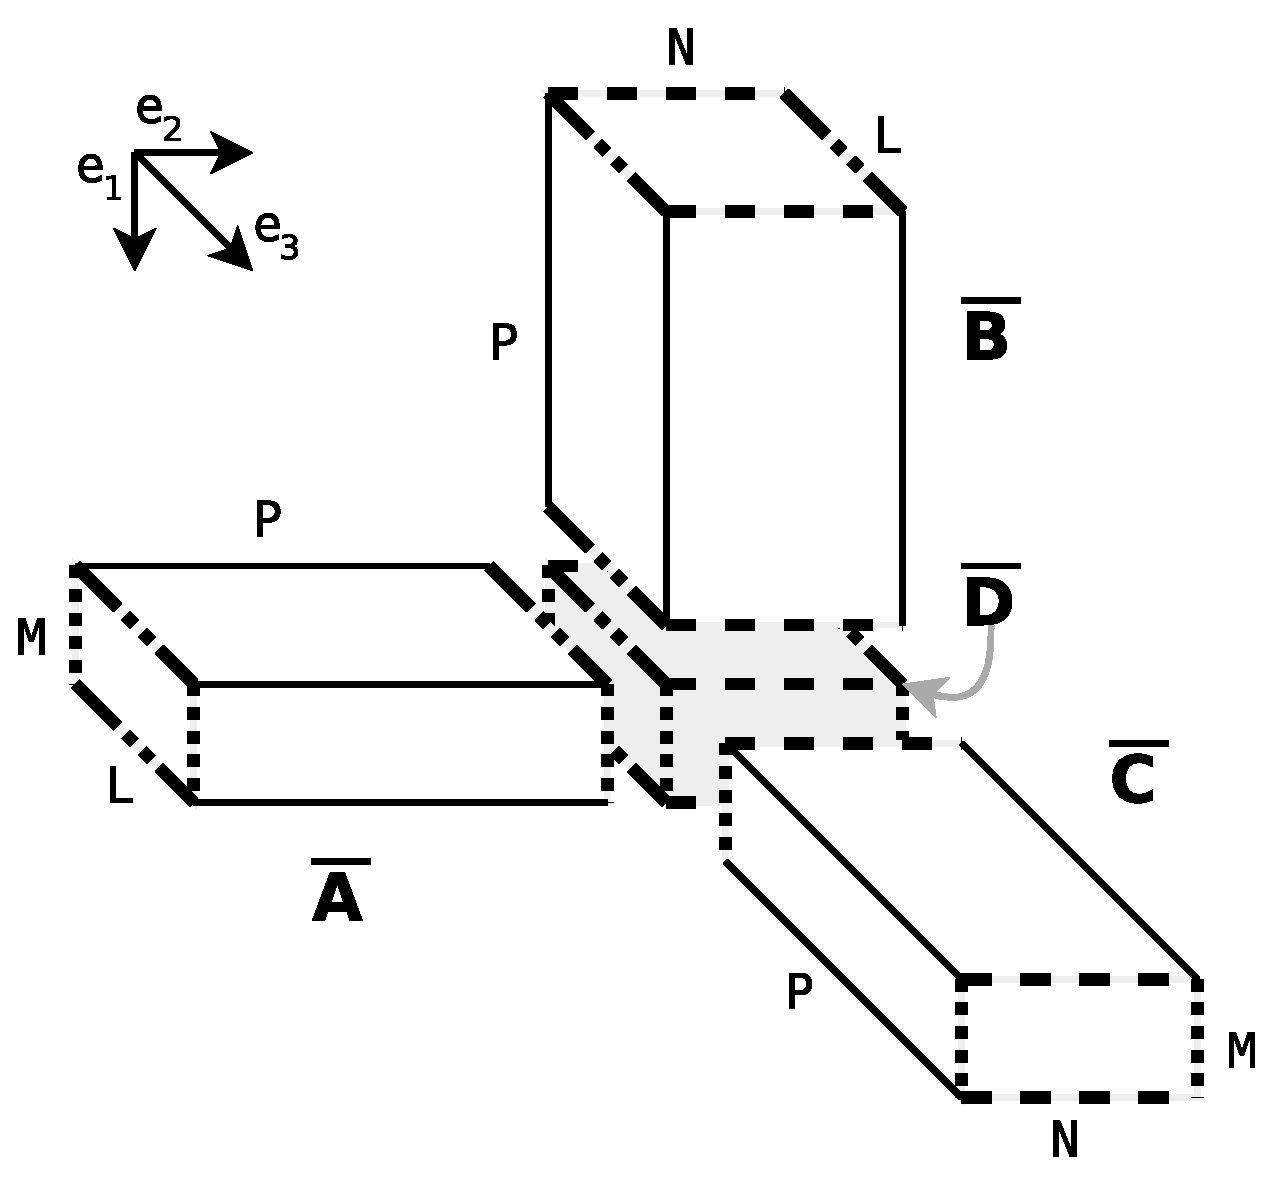
\includegraphics[width=0.8\textwidth]{mulcross3}
    \caption{Cross operation with the trixs $\TRIX{A}$,$\TRIX{B}$ and $\TRIX{C}$.}
    \label{fig:trixcross3C}
\end{figure}

%%%%%%%%%%%%%%%%%%%%%%%%%%%%%%%%%%%%%%%%%%%%%%%%%%%%%%%%%%%%%%%%%%%%%%%%%%%%%%%%%%%%%%%%%%%%%%%%%
%%%%%%%%%%%%%%%%%%%%%%%%%%%%%%%%%%%%%%%%%%%%%%%%%%%%%%%%%%%%%%%%%%%%%%%%%%%%%%%%%%%%%%%%%%%%%%%%%
%%%%%%%%%%%%%%%%%%%%%%%%%%%%%%%%%%%%%%%%%%%%%%%%%%%%%%%%%%%%%%%%%%%%%%%%%%%%%%%%%%%%%%%%%%%%%%%%%
\newpage\
\section{Examples}
The Fig. \ref{fig:trix1} represents a trix $\TRIX{A}\in \mathbb{R}^{4\dimsep 3\dimsep 2}$.
\begin{figure}[h]
  \centering
    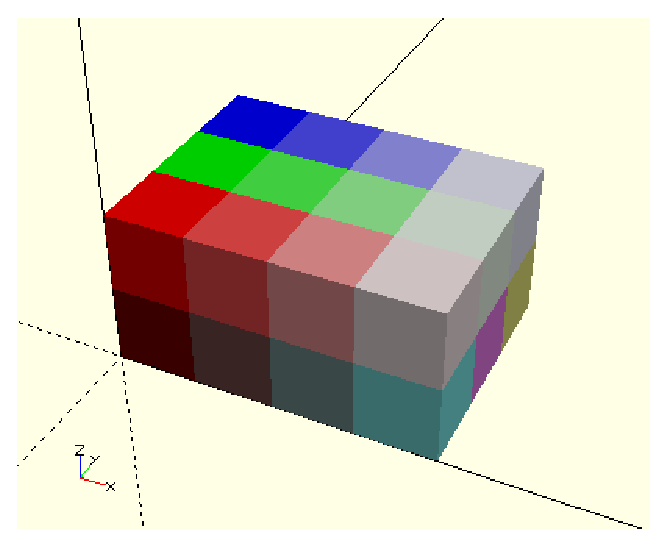
\includegraphics[width=0.2\textwidth]{array3d}
    \caption{Trix A}
    \label{fig:trix1}
\end{figure}

\end{document}
